\documentclass[10pt,conference,compsocconf]{IEEEtran}

\usepackage{hyperref}
\usepackage{graphicx}	% For figure environment
\usepackage{verbatim}
\usepackage{multirow}
\usepackage{amsmath}
\usepackage{algorithm}
\usepackage[noend]{algpseudocode}
%\usepackage{ulem}
\usepackage{dblfloatfix}    % To enable figures at the bottom of page
\usepackage{xcolor}
\definecolor{ao}{rgb}{0.0, 0.5, 0.0}
\usepackage{cprotect}
\usepackage[right=1.5cm, left=1.5cm, top=2cm, bottom=2cm]{geometry}

\begin{document}
\title{81 - Higgs Boson Machine Learning Project}

\author{
  Gael Lederrey, Qendresa Parduzi \& Aidasadat Mousavifar \\
  \textit{EPFL - CS-433 (\emph{Pattern Classification and Machine Learning})}
}

\maketitle

\begin{abstract}

Machine learning techniques have become important and useful tools in resolving questions in different scientific disciplines. The often complex and high dimensional data sets generated in experiments are hard to analyse and interpret. This report gives an overview on the performances of six different machine learning algorithms. Furthermore, it proposes a concrete methodology to approach the problem of binary classification on a real life data-set from CERN.
\end{abstract}

\section{Introduction}
\label{sec:introduction}

The Higgs Boson is an elementary particle which explains why other particles have mass. It was discovered in collision experiments which generated a big amount of data. One example is the Higgs Boson data-set taken from the Atlas experience at CERN. Data-sets like these were used to distinguish signals of the Higgs Boson from background noise. The aim of this project is to use machine learning algorithms in order to find the best approach to complete this taks. We will first implement six basic machine learning algorithms. One of these algorithms will then be further developed into a methodology, which can be used to predict the presence of the Higgs Boson.

\section{Models and Methods}
\label{sec:models_and_methods}

\subsection{Implementation of the mandatory algorithms}
\label{subsec:test}
The six methods (see Table \ref{tab:test_mandatory}) were implemented based on the algorithms presented in the lecture notes.
Depicted in Table \ref{tab:test_mandatory} are the performances of the six mandatory algorithms, which were applied on the training data-set. The parameters $\lambda$ and $\gamma$ have been chosen randomly, \emph{i.e.} without any optimisation. The methods were trained on 80\% of the training data-set and tested on the remaining 20\%.

\begin{table}[h!]
    \centering
    \begin{tabular}{l|c|c|c||c}
        \cline{2-4}
        \multicolumn{1}{}{} & \multicolumn{3}{|c|}{Parameters used} & \multicolumn{1}{}{} \\ \cline{2-4}
        Methods & $\lambda$ & $\gamma$ & \multicolumn{1}{|c|}{max\_iter} & Pred (\%) \\ \hline \hline
        Gradient Descent            & /         & 0.1       & 300   & 74.35\\ 
        Stochastic Gradient Descent & /         & $10^{-3}$ & 300   & 73.25\\
        Least Squares               & /         & /         & /     & 74.47\\
        Ridge Regression            & $10^{-8}$ & /         & /     & 74.47\\
        Logistic Regression         & /         & $10^{-6}$ & 2000  & 75.01\\ 
        Reg Logistic Regression     & 1         & $10^{-6}$ & 2000  & 75.01\\ 
    \end{tabular}
    \caption{Test of the six mandatory algorithms.}
    \label{tab:test_mandatory}
\end{table}

\begin{table*}[!b]
    \centering
    \begin{tabular}{|l|c||c|c|c|c|c|c|c||c|}
        \cline{2-10} 
        \multicolumn{1}{}{} & \multicolumn{9}{|c|}{Correct Prediction (\%)} \\ \cline{2-10}
        \multicolumn{1}{c|}{} & Poly & $CT$ & $\sqrt{CT}$ & $CT^2$ & \multicolumn{4}{c||}{Combinations of Cross-Terms} & Best \\ \cline{1-9}
        Data-sets & (0) & (1) & (2)  & (3) & (1) + (2) & (1) + (3) & (2) + (3) & (1) + (2) + (3) & {\bf \color{ao} 84.20} \\ \hline \hline
        Jet 0 without mass  & 95.02 & 95.13 & {\bf \color{ao} 95.14} & 95.03 & /     & /     & /     & /     & 95.14 \\ 
        Jet 0 with mass     & 80.87 & 81.21 & 80.94 & 81.00 & 81.31 & 81.32 & 81.33 & {\bf \color{ao} 81.40} & 81.40 \\
        Jet 1 without mass  & 92.17 & 92.58 & {\bf \color{ao} 92.83} & 92.78 & /     & /     & /     & /     & 92.83 \\
        Jet 1 with mass     & 79.35 & 79.89 & 79.98 & 79.83 & 80.01 & 80.26 & 80.18 & {\bf \color{ao} 80.49} & 80.49 \\
        Jet 2 without mass  & 92.04 & {\bf \color{ao} 94.68} & 94.55 & 94.55 & /     & /     & /     & /     & 94.68 \\
        Jet 2 with mass     & 83.19 & 84.27 & 84.38 & 83.95 & 84.92 & 84.73 & 84.71 & {\bf \color{ao} 85.34} & 85.34 \\
        Jet 3 without mass  & 94.79 & 97.16 & 97.50 & {\bf \color{ao} 97.83} & /     & /     & /     & /     & 97.83 \\  
        Jet 3 with mass     & 82.89 & 84.00 & 84.31 & 83.88 & {\bf \color{ao} 84.69} & 84.68 & 84.68 & 33.19 & 84.69 \\ \hline \hline
    \end{tabular}
    \caption{Results after training and testing on the train data-set. The Polynomial (0) is always added to the cross-terms. \newline The combinations of cross-terms for the data-sets without mass were not done due to high change of over-fitting.}
    \label{tab:results}
\end{table*}
\vspace{-0.5cm}
In general all the methods are close in their prediction accuracy ranging from 73.25\% - 75.01\%. We can see that on the raw data-set the Logistic Regression methods work best. The Gradient Descent methods are less accurate, whereas the Least Square and the Ridge Regression take an intermediate position. Due to technical difficulties while implementing the Logistic Regression, which were resolved at the end of the project, we decided to proceed with the \emph{Ridge Regression}. We chose the Ridge Regression over the Least Squares to avoid over-fitting and balance the bias and variance with the help of the penalty term $\lambda$.

\subsection{Analysis and preprocessing of the data-sets}

In the exploratory data analysis, we first verified that the distributions of the features are the same for the training and the test set. While looking at the distributions of the features, we see two interesting aspects of the data:
\begin{enumerate}
    \item There are a lot of \emph{NaN} (-999) values in the data.
    \item The feature \verb|PRI_jet_num| takes only four different integer values.
\end{enumerate}

Figure \ref{fig:hist_jet} shows the distribution for the test and the training sets. This result can easily be explained with the physics behind: When two (or more) particles collide they can either create other particles (jets) or destroy each other. Thus it is clear that the number of jets only take integer values. We categorised the data by the number of jets and therefore we could remove this feature vector.

\vspace{-0.5cm}
\begin{figure}[h!]
    \centering
    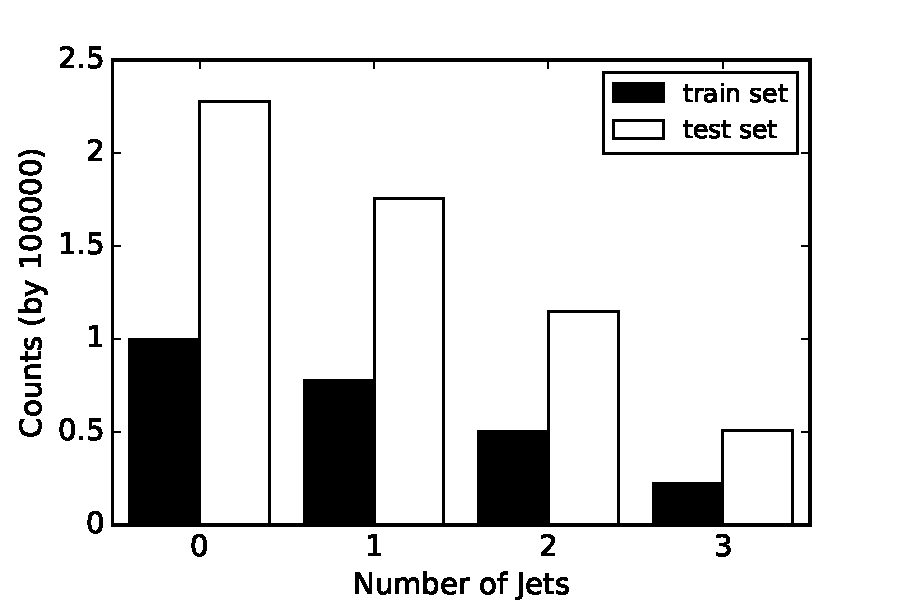
\includegraphics[width=0.9\columnwidth]{hist_jets.pdf}
    \cprotect\caption{Histograms of the feature called \verb|PRI_jet_num| for the test set and train set.}
    \label{fig:hist_jet}
\end{figure} 

In further exploration we observe that features with a lot of \emph{NaN} values often denote angles between the jets.  To assess the validity of the features we check the percentage of \emph{NaN} values for each feature for the four different jets (see Table \ref{tab:nan}). The aforementioned splitting of the data-sets by jets allows us now the removal of several \emph{NaN} containing features. Additionally, we see that the feature \verb|PRI_jet_all| is always zero for jet 0. In order to remove the \emph{NaN} in \verb|DER_mass_MMC| we split the four data-sets again by two: the data with valid values in \verb|DER_mass_MMC| and the data with \emph{NaN}, which will again be removed. For jet 0, we remove all the columns containing \emph{NaN} and the column containing zeros. For jet 1, we remove the columns with \emph{NaN}. We finally end up with eight data-sets without any \emph{NaN} values. 

\begin{table}[h!]
    \centering
    \begin{tabular}{|l||c|c|c|c|}
        \cline{2-5}
        \multicolumn{1}{}{} & \multicolumn{4}{|c|}{Percentage of \emph{NaN}} \\ \hline
        Features with \emph{NaN} & Jet 0 & Jet 1 & Jet 2 & Jet 3 \\ \hline \hline
         \verb|DER_mass_MMC| & 26 & 9 & 5 & 6 \\
         \verb|DER_deltaeta_jet_jet| & 100 & 100 & / & / \\
         \verb|DER_mass_jet_jet| & 100 & 100 & / & / \\
         \verb|DER_lep_eta_centrality| & 100 & 100 & / & / \\
         \verb|PRI_jet_leading_pt| & 100 & / & / & / \\
         \verb|PRI_jet_leading_eta| & 100 & / & / & / \\ 
         \verb|PRI_jet_leading_phi| & 100 & / & / & / \\ 
         \verb|PRI_jet_subleading_pt| & 100 & 100 & / & / \\ 
         \verb|PRI_jet_subleading_eta| & 100 & 100 & / & / \\
         \verb|PRI_jet_subleading_phi| & 100 & 100 & / & / \\ \hline
    \end{tabular}
    \caption{Percentage of \emph{NaN} in the training per jet and per feature. The feature with 0\% of \emph{NaN} are not shown.\vspace{-0.8cm}}
    \label{tab:nan}
\end{table}
\subsection{Cross-Validation}

As mentioned in section \ref{subsec:test}, we will use the Ridge Regression method for training and predicting the Higgs Bosons. For this algorithm, we need to find two parameters: the penalty $\lambda$ and the degree $d$ for the polynomial basis. We used a 10-fold cross-validation on the training set to obtain the parameters given in Table \ref{tab:cv}. Instead of using the minimum value of the average losses on the $k$-folds, we use the minimum of the median value due to many outliers.  

\begin{table}[h!]
    \centering
    \begin{tabular}{|l||c|c|}
        \hline
        Data-sets & $\lambda$ & degree \\ \hline\hline
        Jet 0 without mass & $9.00\cdot10^{-6}$ & 12 \\ \hline
        Jet 0 with mass & $2.12\cdot10^{-2}$ & 9 \\ \hline
        Jet 1 without mass & $1.65\cdot10^{-5}$ & 7 \\ \hline
        Jet 1 with mass & $2.70\cdot10^{-4}$ & 9 \\ \hline
        Jet 2 without mass & $2.42\cdot10^{-6}$ & 10 \\ \hline
        Jet 2 with mass & $3.09\cdot10^{-2}$ & 10 \\ \hline
        Jet 3 without mass & $4.00\cdot10^{-5}$ & 8 \\ \hline
        Jet 3 with mass & $3.63\cdot10^{-10}$ & 9 \\ \hline
    \end{tabular}
    \caption{Parameters obtained with the 10-fold Cross-Validation.\vspace{-0.8cm}}
    \label{tab:cv}
\end{table} 

\subsection{Adding Features}
\label{sec:cross-terms}

In Physics (more precisely in Particle Physics), the mass, the angles and, the energies are related to each other with different degrees, \emph{i.e.} there are non-linear relationships between parameters. So, we decided to add cross-terms by pairs to the matrix of samples in the polynomial basis. Nevertheless, we did not perform the cross-validation on this new sample matrix due to time constraints. Table \ref{tab:results} shows all the combinations of cross-terms we used:
\begin{itemize}
    \item $CT$: Multiplications by pairs of the columns of $X$
    \item $\sqrt{CT}$: Square root of the multiplications
    \item $CT^2$: Multiplications squared
\end{itemize}

\subsection{Training and Test}
We compute the new matrix of samples using the best degree found with the cross-validation and adding the right cross-terms. We simply apply the Ridge Regression with the best penalty $\lambda$ to obtain the optimal weights, with which we compute the prediction on the testing data. The final step is to aggregate the predictions of the eight data-sets together.

\section{Results and Discussion}

The prediction results of the mandatory algorithms were in accordance to our expectations, with the Logistic Regressions being the optimal methods to do binary classifications. Nevertheless all the methods yield similar prediction results.

For the developed methodology, we need to discuss the results of the cross-validation. We see the tendency that the polynomial degrees differ between the data-sets depending whether the mass is present or not. Since the data-sets without mass have less features, we expect easier models, thus less polynomial degrees, to achieve a good prediction. It is true for all jets but the first one, where the cross-validation yields a higher degree. Additionally, we did not add many cross-terms on the data-sets without the mass, since due to its small size this would lead to overfitting.
With our method we achieved a total of 83.544\% of overall correct prediction in the Public Leaderboard on Kaggle. Looking at the smaller models (see Table \ref{tab:results}), we observe different results. This might be due to slight overfitting, which is nevertheless limited by the penalty parameter $\lambda$.

\section{Conclusion}

We saw in this project that we can use various algorithms to train on data to do a binary classification. Even though we proceeded with the Ridge Regression, the Logistic Regression would be a reasonable choice as well. We learned that preprocessing the data is essential in order to achieve good predictions. In this project we decided to remove \emph{NaN} values, but there are many ways to deal with missing values, such as replacing them with the correct distribution, which might lead even to better predictions. 


%\bibliographystyle{IEEEtran}
%\bibliography{literature}

\end{document}